\subsection{Air Pollution Monitoring Sensors}
Over the last century world-wide energy consumption has increased at a rapid rate due to industrialization, economic and population growth. As a result, the world has also seen an evident spike in the levels of polluting gases emitted in the air which can have detrimental effects to the environment and humans. The burning of fossil fuels for energy consumption leads to the emissions of Carbon Dioxide (CO2) and other harmful gases such as Carbon Monoxide (CO), Nitrogen Oxides (\nox), Sulfur Dioxide (SO2), and Particulate Matters (PM2.5 and PM10) all of which are harmful toxins. Air pollution monitoring systems have been developed to track these emissions and ensure air quality and enforce environmental standards.These systems are based on sophisticated equipment that measure air quality and can detect gases and matters using a variety of methods. In this section and the following subsections, the different types of sensors that are available and the methods they use to track pollutants are discussed. The sensors that were considered and chosen for the Aether air pollution sensor network are also discussed here. These sensors were chosen based on several factors including cost, accuracy, integration, and power consumption. Table \ref{gas-sensor-comparison} shows the comparison of these type of sensors.


\subsubsection{Environmental Gas Sensor}
There are mainly 5 different types of gas sensors which use different methods to detect gases, each with their own advantages and disadvantages. The most widely used gas sensors today are electrochemical sensors, catalytic sensors, solid-state semiconductor sensors, non-dispersive infrared (NDIR) and photo-ionization detector (PID) sensors. Due to the constant interaction of different gasses in the air, individual gas sensors have to be calibrated more than other kinds of sensors. Sensors will need to be exposed to a pre-determined pollutant with a specified concentration so the difference between gas concentration and sensor reading is minimized. Although portable and low cost, these sensors cannot achieve the level of accuracy as other industrial grade measuring systems but can however be accurate enough to detect dangerous levels of toxic and polluting gases used to calculate AQI levels. Four gases are the primary contributors to poor air quality and are the ones mainly used in calculating the AQI index, CO, NO2, O3, and SO2. The type of gas sensors best fitted to detect these gases are listed below. 

\begin{itemize}
    \item \ozone: Is best detected by electrochemical and solid-state sensors
    \item \sdo: Only detectable with electrochemical and solid-state sensors as NDIR sensors aren’t sensitive enough and catalytic sensors would be burned with the toxins
    \item \nox : Is best detected by electrochemical and solid-state sensors; readings easily interfered by the presence of O3 
    \item CO: Detected by electrochemical and solid-state sensors
\end{itemize}
In the research conducted for finding the most suitable sensors for Aether, it was determined that electrochemical sensors were the most reasonable in price and power consumption while still providing reliable and accurate readings for measuring air quality in outdoor and indoor uses. The operating mechanisms of each type of gas sensor is discussed below. 

\paragraph{Solid-state Gas Sensors}
The working principle behind solid-state gas sensors was discovered around the same time when research was being conducted on p-n junction devices. Solid-state sensors typically have one or more transition metal oxide with a heating element which regulates the temperature of the sensor. The metal oxide causes the gas particles to dissipate into charged particles resulting in the transfer of electrons. There is a circuit which regulates the heating element to operate at the sensor’s specific temperature range where gas can be optimally detected. Electrodes integrated into the metal oxide cause a change in conductivity due to the molecular interaction of gas particles. In turn, this change in conductivity is measured as a signal relating to the level of gas concentration. 

Solid-state sensors have appealing characteristics as they provide a high degree of versatility and longevity. Due to the operating mechanisms behind these types of sensors, with the right filtering in place to block out certain gases, solid state devices can be made to detect a over 150 different type of gases. Additionally, another major advantage of solid-state sensors is the lifespan, with an average life expectancy of over 10 years it makes it an ideal candidate for long-term low maintenance use. 

\paragraph{Electrochemical Gas Sensors}
The operating mechanisms behind electrochemical gas sensing are electrochemical reactions, specifically oxidation and reduction reactions. With working electrodes in place, the reaction of gas molecules with ambient oxygen particles generates an output current proportional to the level of gas concentration present. The output current is then converted to a parts per million (PPM) unit. The type of electrodes and membranes used within the circuit are determined by the type of gas the sensor is trying to detect. 

Electrochemical sensors have the lowest power consumption of any other kind of gas sensor making it an ideal candidate for use in the Aether sensor network system. The response times for these sensors are usually under 50 seconds and the typical life span ranges anywhere from 2 to 3 years. When compared to solid-state sensors, there is a trade off between cost and accuracy. Although not nearly as accurate as industrial grade solid-state devices, it still generates an accurate enough reading to calculate ambient air quality and gas concentrations at a tenth of the price, with most electrochemical sensors ranging any where from a few dollars to 50 dollars. 
	
\paragraph{Catalytic Gas Sensors}
Catalytic-type gas sensors consist of a detector element that burns in the presence of combustible gases causing a rise in temperature and thus a rise in resistance. The change in resistance is proportional to the level of  combustible gas present. Combustible gases include methane, propane, and hydrogen. Since the gases fall outside of the gases contributing to poor air quality, specific catalytic sensors were not considered for the development of this product design

\begin{figure}
    \centering
    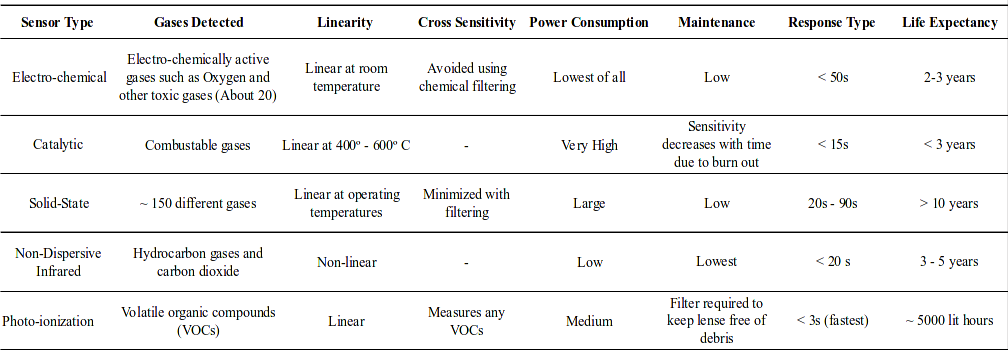
\includegraphics[width=6in]{figures/gas-sensor-comparison.png}
    \caption{A comparison of the different features of gas sensors.}
    \label{gas-sensor-comparison}
\end{figure}


% \begin{table}[H]
% \centering
% \footnotesize	
% \begin{tabularx}{\linewidth}{|X X X X X|}
% \hline
% Sensor Type & Gases Detected & Linearity & Cross Sensitivity & Power Consumption  \\\hline\hline
% Electro-chemical & Electro-chemically active gases such as oxygen and other toxic gasses (about 20) & Linear at room temperature & Avoided using chemical filtering & Lowest of all \\
% Catalytic & Combustable gases & Linear at $400\deg - 600\deg$ C & - & Very high \\ 
% \end{tabularx}
% \vspace{1 cm}
% \begin{tabular}{c c c}
% \hline
% Maintenance & Response Type & Life Expectancy \\\hline\hline
% \end{tabular}



% \label{Gases}
% \caption{Gases}
% \end{table}
\subsubsection{Particulate Matter Sensor}

\subsubsection{VOC and VSC Sensor}

\subsubsection{Sensors Used In Aether}
